\documentclass[10pt,t,aspectratio=169]{beamer}
%\usetheme{Berkeley}
\usepackage{graphicx}
\usepackage{amsmath}
\usepackage[american]{circuitikz}

% Packages to plot functions
\usepackage{pgfplots}
\pgfplotsset{compat=newest}

\usepackage{multicol}
\usepackage{multirow}
\usepackage{textcomp} % to use \textmu
\usepackage[absolute,overlay]{textpos} % to place floating text boxes with \begin{textblock*}{width}(x,y)
\usepackage{tcolorbox}
\usepackage{colortbl} % allows coloring cells of a table with \cellcolor{blue!25}

\title{Clase 6}
\subtitle{Contactos metal-semiconductor}
\author{Dr.-Ing. Juan José Montero Rodríguez}
\subject{Elementos Activos}
\institute{Escuela de Ingeniería Electrónica}
\date{Semestre II-2023}
\titlegraphic{
\includegraphics[height=12mm]{figures/logoTEC.pdf}}


\begin{document}

\begin{frame}[t]
\titlepage
\end{frame}




\begin{frame}[t]
    \frametitle{Contactos M-S: Contacto Óhmico y Contacto Schottky}

    \begin{itemize}
        \item La unión de un metal con un semiconductor produce contactos con las siguientes curvas de transferencia I-V:
    \end{itemize}

    \begin{columns}
        \begin{column}{0.5\textwidth}
            \centering
            \textbf{Contacto Óhmico}

            \begin{figure}[H]
                \centering
                \pgfplotsset{width=\textwidth,compat=1.9}
                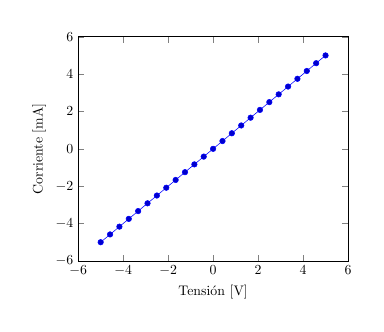
\begin{tikzpicture}[scale = 0.5]
                  \begin{axis}[ 
                    xlabel={Tensión [V]},
                    ylabel={Corriente [mA]}
                    ] 
                    \addplot{x}; 
                  \end{axis}
                \end{tikzpicture}
                \end{figure}

                \flushleft
                Aplicaciones:

                \begin{itemize}
                    \item Conexión entre el semiconductor y terminales metálicas de dispositivos electrónicos.
                \end{itemize}
        \end{column}
        \begin{column}{0.5\textwidth}
            \centering
            \textbf{Contacto Schottky}

            \begin{figure}[H]
                \centering
                \pgfplotsset{width=\textwidth,compat=1.9}
                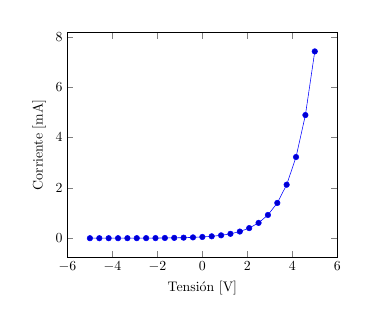
\begin{tikzpicture}[scale = 0.5]
                  \begin{axis}[ 
                    xlabel={Tensión [V]},
                    ylabel={Corriente [mA]}
                    ] 
                    \addplot{0.05*e^x};  
                  \end{axis}
                \end{tikzpicture}
            \end{figure}

            \flushleft
            Aplicaciones:

            \begin{itemize}
                \item Rectificación
                \item Diodos de alta velocidad
            \end{itemize}
        \end{column}
    \end{columns}
\end{frame}


\begin{frame}[t]
    \frametitle{Contacto Óhmico y Contacto Schottky}

    \begin{itemize}
        \item Al unir un metal con un semiconductor, existen cuatro posibilidades:
        \begin{itemize}
            \item Metal puede tener $\phi_M$ mayor o menor que $\phi_S$.
            \item Semiconductor puede ser de \textbf{tipo n} o \textbf{tipo p}.
        \end{itemize}
        \vspace{3mm}
        \item Las cuatro combinaciones posibles se resumen en la siguiente tabla:
        \begin{tabular}{ccc}
            \hline
            \textbf{Condición} & \textbf{Metal-Semi n} & \textbf{Metal-Semi p} \\
            \hline
            $\phi_M > \phi_S$ & Schottky & Óhmico \\
            $\phi_M < \phi_S$ & Óhmico & Schottky \\
            \hline
        \end{tabular}
        \vspace{3mm}
        \item \textbf{El contacto óhmico es un contacto no rectificante:}
        \begin{itemize}
            \item Conducción es posible en ambos sentidos: directo e inverso.
            \item Se comporta como una resistencia en ambas direcciones.
        \end{itemize}
        \vspace{3mm}
        \item \textbf{El contacto Schottky es un contacto rectificante:}
        \begin{itemize}
            \item Conducción es posible en sentido directo (una sola dirección).
            \item En sentido inverso no hay posibilidad de conducción.
        \end{itemize}
    \end{itemize}
\end{frame}


\begin{frame}[t]
    \frametitle{Contacto Óhmico y Contacto Schottky}

    Los siguientes son ejemplos de los tipos de contactos:

    \vspace{3mm}
    \begin{columns}
        \begin{column}{0.33\textwidth}
            1) Contacto Schottky Si-n
            
            \[\boxed{\phi_M > \phi_S}\]

            \centering
            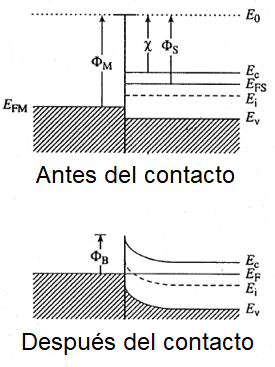
\includegraphics[width=3.5cm]{./figures/contactos1.png}
        \end{column}
        \begin{column}{0.33\textwidth}
            2) Contacto Óhmico Si-n
            
            \[\boxed{\phi_M < \phi_S}\]

            \centering
            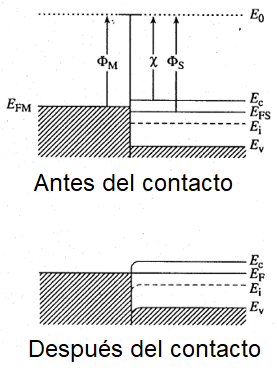
\includegraphics[width=3.5cm]{./figures/contactos2.png}
        \end{column}
        \begin{column}{0.33\textwidth}
            3) Contacto Schottky Si-p

            \centering
            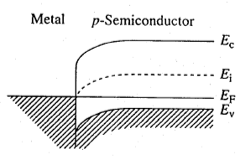
\includegraphics[width=3.5cm]{./figures/contactos3.png}

            \flushleft\vspace{5mm}
            4) Contacto Óhmico Si-p

            \centering
            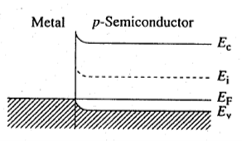
\includegraphics[width=3.5cm]{./figures/contactos4.png}
        \end{column}
    \end{columns}
\end{frame}


\begin{frame}[t]
    \frametitle{Caso 1:	Metal-Silicio N \hspace{1cm} $\phi_M>\phi_S$ \hspace{1cm} (Schottky)}

    \begin{columns}
    
        \begin{column}{0.5\textwidth}
        
            \centering
            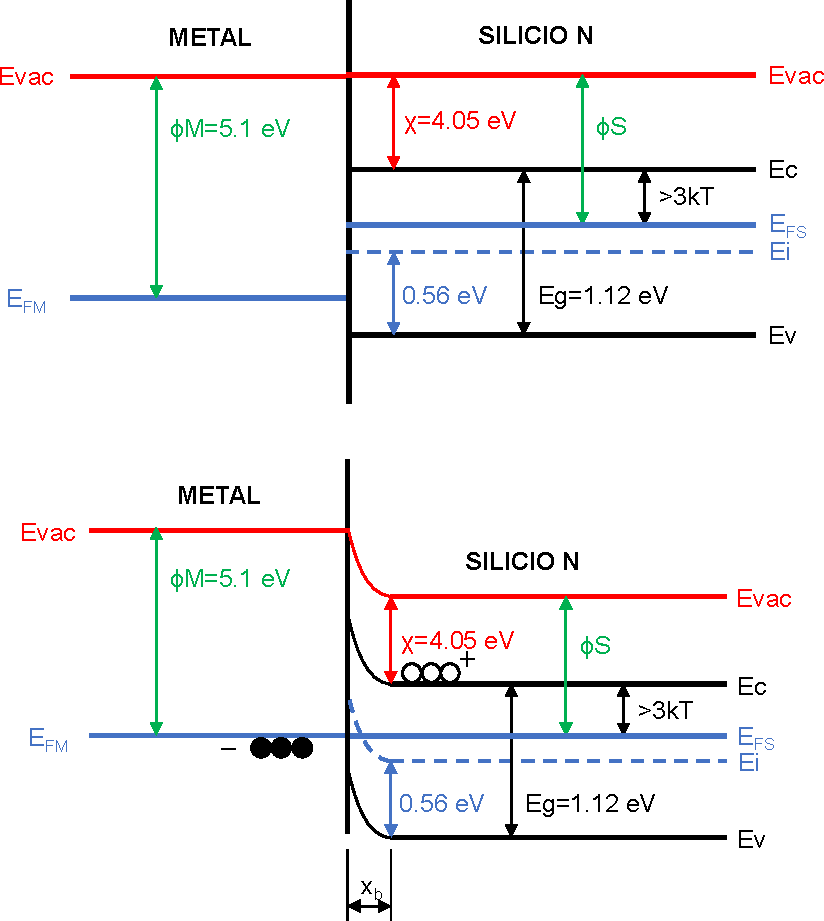
\includegraphics[height=7cm]{./figures/contactos-caso1.pdf}
            
        \end{column}
        
        \begin{column}{0.5\textwidth}
        
            \begin{itemize}
                \item Al unir ambos materiales, el nivel de Fermi del metal se alinea con el nivel de Fermi del semiconductor.
                \item Los niveles de energía del semiconductor cambian, se desplazan hacia \textbf{abajo}.
                \item Se produce una diferencia de potencial $\phi_B$ y se crea el potencial de contacto $V_{bi}$
                \item Electrones no pueden fluir del metal al semiconductor.
            \end{itemize}

            \vspace{5mm}
            \centering
            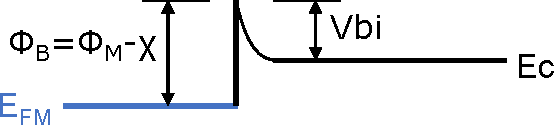
\includegraphics[width=5cm]{./figures/contactos-caso1b.pdf}
            %
            \[ V_{bi} = \dfrac{1}{q}(\phi_M - \phi_S) = \dfrac{1}{q}(\phi_B - (E_C - E_F)) \]
            
        \end{column}

    \end{columns}
    
\end{frame}



\begin{frame}[t]
    \frametitle{Caso 2:	Metal-Silicio N \hspace{1cm} $\phi_M<\phi_S$ \hspace{1cm} (Óhmico)}

    \begin{columns}
    
        \begin{column}{0.5\textwidth}
        
            \centering
            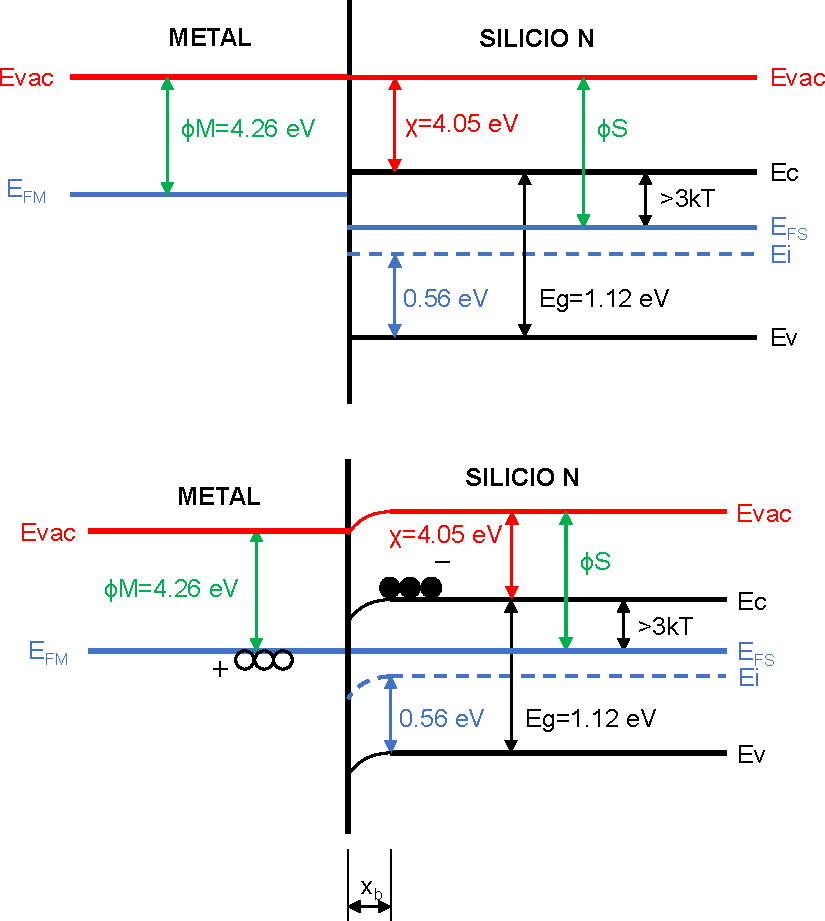
\includegraphics[height=7cm]{./figures/contactos-caso2.pdf}
            
        \end{column}
        
        \begin{column}{0.5\textwidth}
        
            \begin{itemize}
                \item Al unir ambos materiales, el nivel de Fermi del metal se alinea con el nivel de Fermi del semiconductor.
                \item Los niveles de energía del semiconductor cambian, se desplazan hacia \textbf{arriba}.
                \item La barrera de potencial es muy pequeña para los electrones del metal. El potencial de contacto no existe.
                \item Electrones fluyen en ambas direcciones.
            \end{itemize}

            \vspace{5mm}
            \centering
            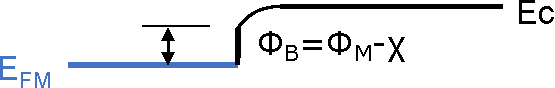
\includegraphics[width=5cm]{./figures/contactos-caso2b.pdf}
            
            
        \end{column}
        
    \end{columns}
    
\end{frame}


\begin{frame}[t]
    \frametitle{Caso 3:	Metal-Silicio P \hspace{1cm} $\phi_M<\phi_S$ \hspace{1cm} (Schottky)}

    \begin{columns}
    
        \begin{column}{0.5\textwidth}
        
            \centering
            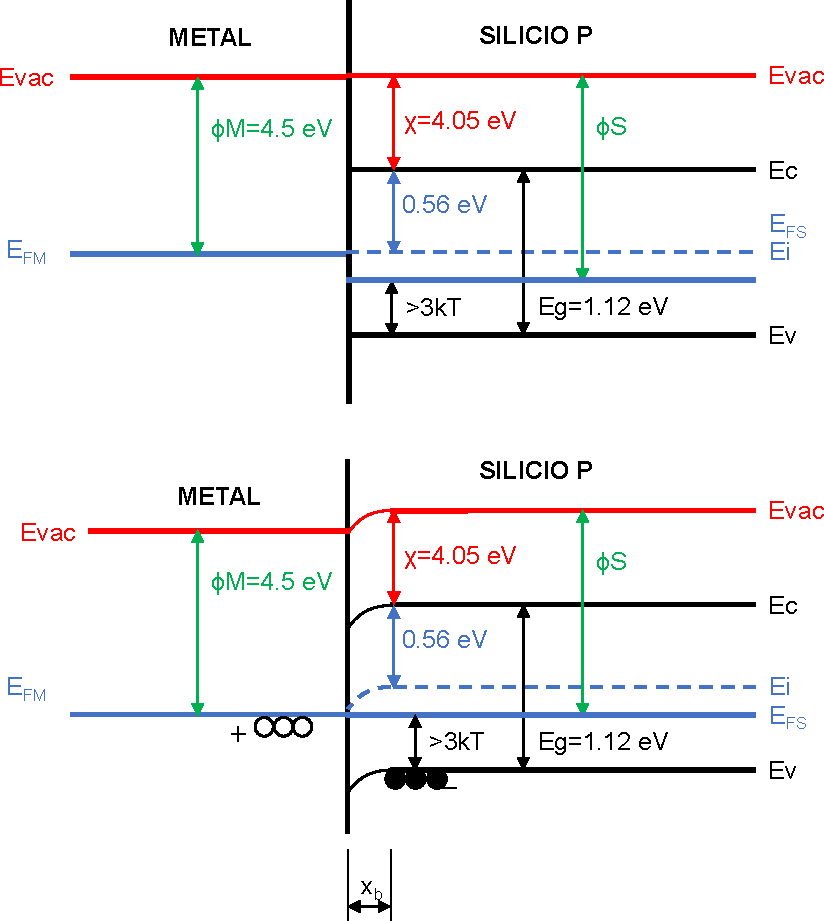
\includegraphics[height=7cm]{./figures/contactos-caso3.pdf}
            
        \end{column}
        
        \begin{column}{0.5\textwidth}
        
            \begin{itemize}
                \item Al unir ambos materiales, el nivel de Fermi del metal se alinea con el nivel de Fermi del semiconductor.
                \item Los niveles de energía del semiconductor cambian, se desplazan hacia \textbf{arriba}.
                \item Se produce una diferencia de potencial $\phi_B$ y se crea el potencial de contacto $V_{bi}$
                \item Huecos no pueden pasar del metal al semiconductor.
            \end{itemize}

            \vspace{5mm}
            \centering
            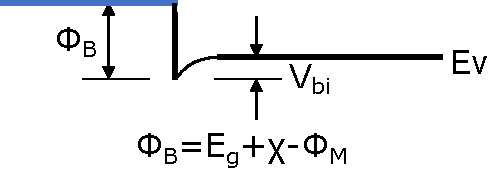
\includegraphics[width=5cm]{./figures/contactos-caso3b.pdf}
            
        \end{column}
        
    \end{columns}
    
\end{frame}


\begin{frame}[t]
    \frametitle{Caso 4:	Metal-Silicio P \hspace{1cm} $\phi_M>\phi_S$ \hspace{1cm} (Óhmico)}

    \begin{columns}
    
        \begin{column}{0.5\textwidth}
        
            \centering
            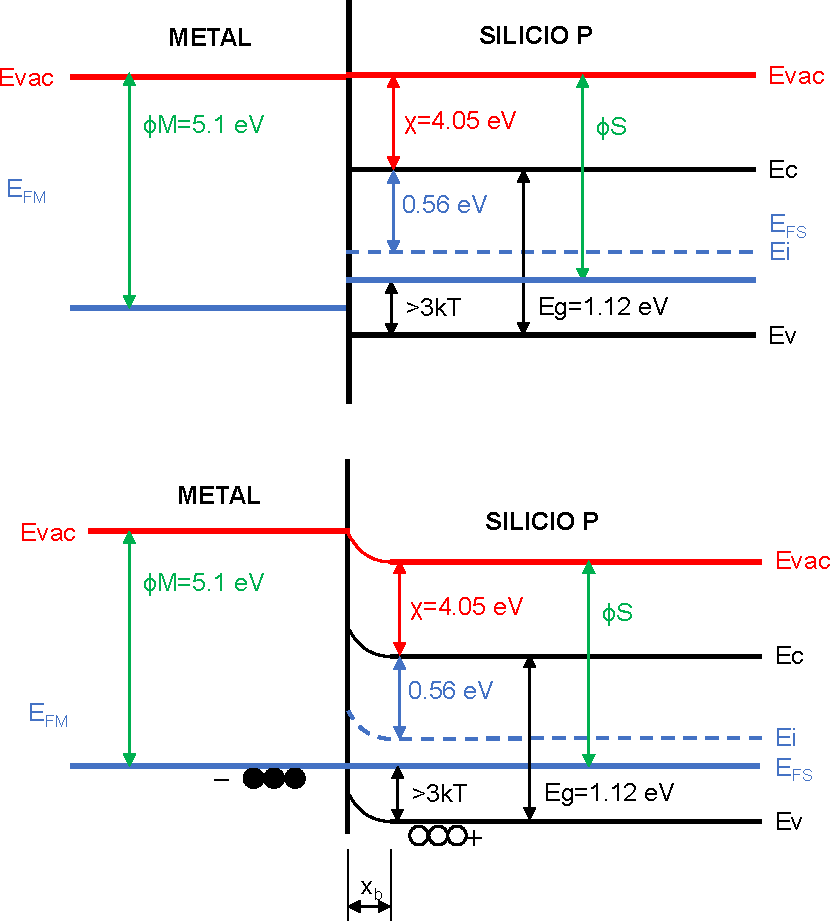
\includegraphics[height=7cm]{./figures/contactos-caso4.pdf}
            
        \end{column}
        
        \begin{column}{0.5\textwidth}
        
            \begin{itemize}
                \item Al unir ambos materiales, el nivel de Fermi del metal se alinea con el nivel de Fermi del semiconductor.
                \item Los niveles de energía del semiconductor cambian, se desplazan hacia \textbf{abajo}.
                \item La barrera de potencial es muy pequeña para los huecos del metal.
                \item El potencial de contacto no existe: huecos pasan en ambas direcciones.
            \end{itemize}

            \vspace{5mm}
            \centering
            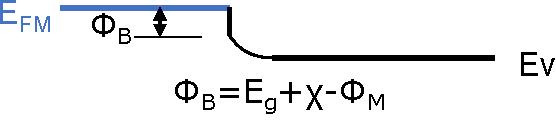
\includegraphics[width=5cm]{./figures/contactos-caso4b.pdf}
            
        \end{column}
        
    \end{columns}
    
\end{frame}


\begin{frame}[t]
    \frametitle{Contacto Schottky con Tensión Aplicada (M-S tipo n)}

    \begin{itemize}
        \item Al aplicar una tensión, los diagramas de bandas se deforman.
        \begin{itemize}
            \item El contacto Schottky bloquea corriente en una dirección.
            \item El contacto Óhmico permite el paso de corriente en ambas direcciones.
        \end{itemize}
    \end{itemize}

    \begin{columns}
    
        \begin{column}{0.4\textwidth}
        
            \centering
            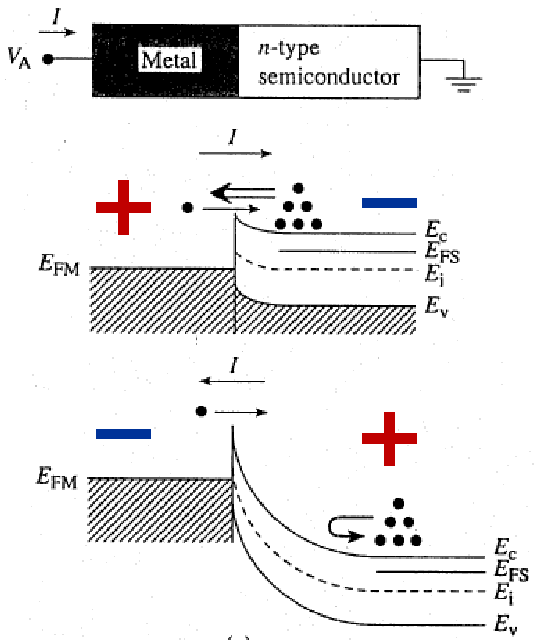
\includegraphics[width=4.5cm]{./figures/contacto-schottky-con-VA.pdf}
            
        \end{column}
        
        \begin{column}{0.6\textwidth}
        
            Considere el contacto que se muestra en la figura de la izquierda.

            \vspace{3mm}
            El ancho de la deformación de bandas $x_b$ cambia con la tensión aplicada.

            \vspace{3mm}
            \begin{itemize}
                \item Si se aplica un potencial $V_A$ positivo (\textbf{polarización directa}, como se muestra en la primera figura) las bandas suben y el ancho de la región $x_b$ \textbf{disminuye}.
                \item Si se aplica un potencial $V_A$ negativo (\textbf{polarización inversa}, como se muestra en la segunda figura), las bandas bajan y el ancho de la región $x_b$ \textbf{aumenta}.
            \end{itemize}
            
        \end{column}
        
    \end{columns}
    
\end{frame}



\begin{frame}[t]
    \frametitle{Electrostática en Contacto Schottky (M-S tipo n)}

\begin{columns}

\begin{column}{0.4\textwidth}

\centering
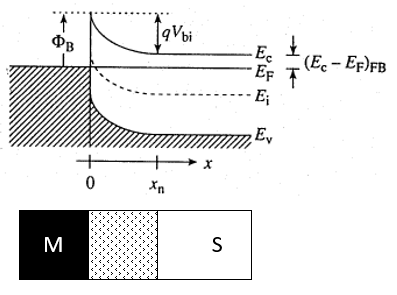
\includegraphics[width=\textwidth]{figures/schottky_electrostatics_1.png}

\flushleft
La región $x_n$ se conoce como región de agotamiento. No hay portadores de carga libres: todos los electrones se pasaron al metal.

\end{column}

\begin{column}{0.18\textwidth}

\centering
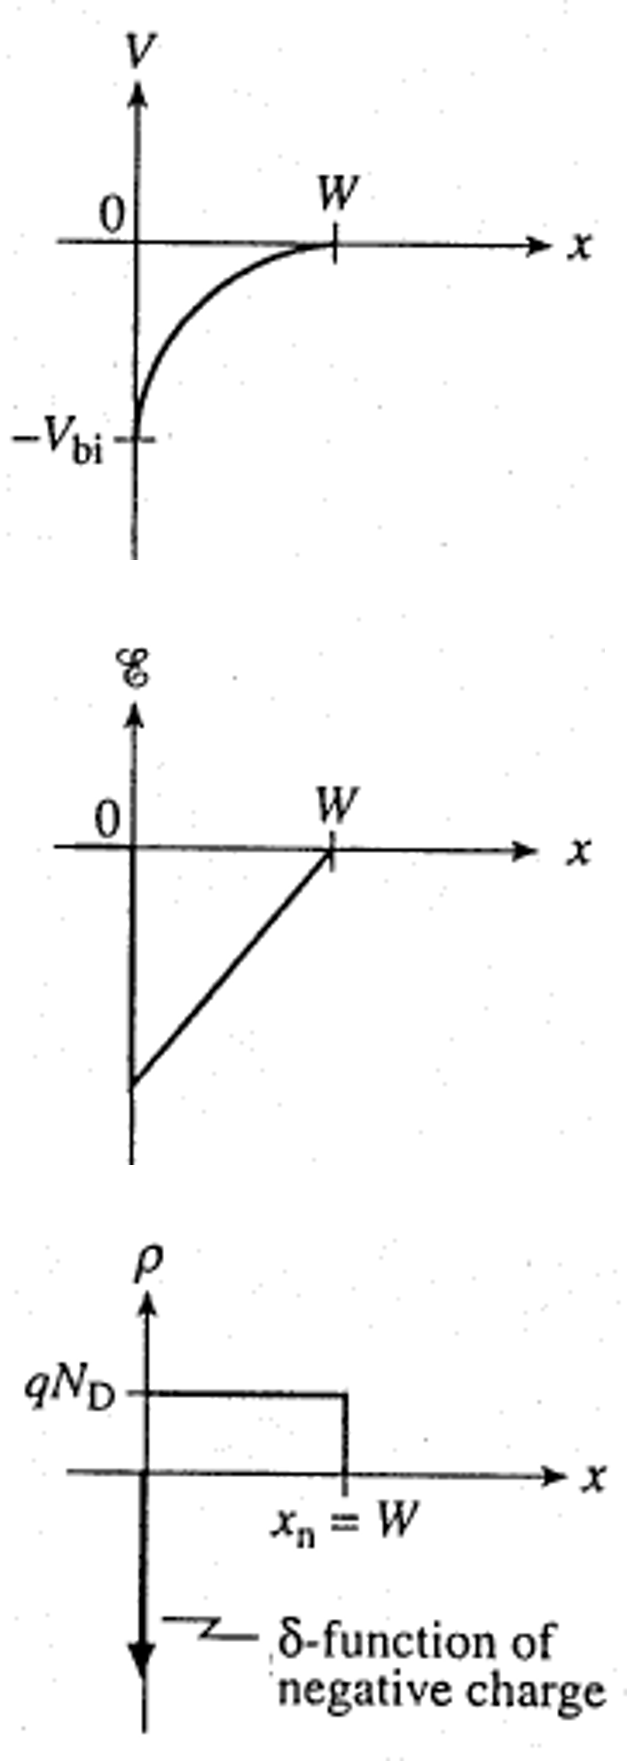
\includegraphics[width=\textwidth]{figures/schottky_electrostatics_2.png}

\end{column}
\begin{column}{0.32\textwidth}

\textbf{1. Potencial}
%
\[ E = -q V \]
%
\[ V = \dfrac{-(E_C - E_{ref})}{q} \]

\textbf{2. Campo eléctrico}
%
\[ \mathcal{E} = \dfrac{-dV}{dx} = \dfrac{1}{q} \dfrac{dE_C}{dx} \]

\textbf{3. Densidad de carga}

La ecuación de Poisson:
%
\[ \dfrac{d\mathcal{E}}{dx} = \dfrac{\rho}{\epsilon_0 \epsilon_r} = \dfrac{q N_D}{\epsilon_0 \epsilon_r} \]

\end{column}
\end{columns}

\end{frame}


\begin{frame}{Ancho de la región de agotamiento (Schottky M-S tipo n)}

\begin{columns}

\begin{column}{0.5\textwidth}

La ecuación de Poisson:
\[ \dfrac{d\mathcal{E}}{dx} = \dfrac{\rho}{\epsilon_0 \epsilon_r} = \dfrac{q N_D}{\epsilon_0 \epsilon_r} \]

Integrando a ambos lados:
\[ \int_{\mathcal{E}}^{0} d\mathcal{E} = \int_x^w \dfrac{q N_D}{\epsilon_0 \epsilon_r} dx \]
\[ \mathcal{E} = \dfrac{-q N_D}{\epsilon_0 \epsilon_r} (w - x) \]

Donde $x$ es una posición arbitraria en el material.

\end{column}

\begin{column}{0.5\textwidth}

El potencial se obtiene al integrar el campo eléctrico:
\[ \dfrac{dV}{dx} = -\mathcal{E} \]
\[ \int_{V(x)}^{0} dV = \int_x^w \dfrac{-q N_D}{\epsilon_0 \epsilon_r} (w - x) dx \]
\[ V(0) - V(x) = \dfrac{-q N_D}{\epsilon_0 \epsilon_r} (w - x)^2 \]

Se despeja el ancho de la zona de agotamiento (con $V(w) = V_{bi}$ y $V(0) = V_A$)
\[ \boxed{w = \sqrt{\dfrac{2 \epsilon_0 \epsilon_r (V_{bi} - V_A)}{q N_D}}} \]

\end{column}

\end{columns}

\end{frame}


\begin{frame}{Capacitancia de directa del diodo Schottky}

Los diodos en reversa son un circuito abierto, y en directa son un corto circuito.

\vspace{5mm}
Sin embargo, el modelo no ideal del diodo involucra resistencia y capacitancia.

\vspace{5mm}
\begin{itemize}
    \item Cuando se polariza en directa, el diodo Schottky tiene una zona de agotamiento con ancho $x_d$.
    \item La densidad de carga existente en la zona de agotamiento es $\rho$.
    \item La permitividad relativa del silicio es $\epsilon_r = 11.9$.
    \item La distancia entre las ``placas'' paralelas de un condensador es $x_d$.
\end{itemize}

\vspace{5mm}
Por lo tanto, la capacitancia del diodo Schottky (por unidad de área) es:

\[ \boxed{C_j = \dfrac{\epsilon_0 \epsilon_r}{w} = \sqrt{\dfrac{q N_D \epsilon_0 \epsilon_r}{2 (V_{bi} - V_A)}}} \]

\end{frame}


\begin{frame}{Ejemplo: Diodo Schottky I}

Se deposita cobre sobre un sustrato cuidadosamente preparado de silicio n, para formar un diodo Schottky ideal. $\phi_M=4.65\ eV$, $\chi=4.03\ eV$, $N_D=10^{16}\ cm^{-3}$ y $T=300\ K$. 

\vspace{5mm}Determine:

\begin{enumerate}
    \item La barrera Schottky $\phi_B$.
    \item El potencial de contacto $V_{bi}$.
    \item El ancho de la región de agotamiento $w$ si $V_A = 0\ V$.
    \item El valor máximo del campo eléctrico $\mathcal{E}$ si $V_A = 0\ V$.
\end{enumerate}

\vspace{5mm}
Referencia: Pierret, p487.
    
\end{frame}


\begin{frame}{Solución: Diodo Schottky I}

Se deposita cobre sobre un sustrato cuidadosamente preparado de silicio n, para formar un diodo Schottky ideal. $\phi_M=4.65\ eV$, $\chi=4.03\ eV$, $N_D=10^{16}\ cm^{-3}$ y $T=300\ K$. 

\begin{columns}

\begin{column}{0.5\textwidth}

1. La barrera Schottky $\phi_B$:

$\phi_B = \phi_M - \chi$

$\phi_B = 4.65\ eV - 4.03\ eV$

$\phi_B = 0.62\ eV$

\vspace{5mm}

2. El potencial de contacto $V_{bi}$:

$E_C - E_F = \dfrac{E_g}{2} - kT \ln \dfrac{N_D}{n_i}$

$E_C - E_F = 0.56\ eV - 26\ meV \ln 10^6$

$E_C - E_F = 0.20\ eV$

$V_{bi} = \dfrac{1}{q} \left[ \phi_B - (E_C - E_F) \right]$

$V_{bi} = \dfrac{1}{q} \left[ 0.62\ eV - 0.20\ eV \right]$

$V_{bi} = 0.42\ V$
\end{column}

\begin{column}{0.5\textwidth}

3. El ancho de la región de agotamiento:
%
\[ w = \sqrt{\dfrac{2(11.9)(8.85\times{}10^{-14})(0.42 - 0)}{(1.6\times{}10^{-19})(10^{16})}} \]
%
\[ w = 0.234\ \mu m \]

\vspace{5mm}
4. El valor máximo del campo eléctrico:
%
$ \mathcal{E}_{max} = \mathcal{E}(0) = \dfrac{q N_D (w - 0)}{\epsilon_0 \epsilon_r} $
%
$ \mathcal{E} = \dfrac{(1.6\times{}10^{-19})(10^{16})(2.34\times{}10^{-5})}{(11.9)(8.85\times{}10^{-14})} $
%
$ \mathcal{E} = 3.59\times{}10^4\ V/cm $

\end{column}

\end{columns}
    
\end{frame}


\begin{frame}{Ejemplo: Diodo Schottky II}

Se tiene una unión de cromo-silicio con $N_D = 10^{17}\ cm^{-3}$.

Se aplica una tensión $V_A = -5\ V$ en la terminal del metal.

La terminal del semiconductor está conectada a tierra.

\vspace{5mm}
Calcule:

\begin{enumerate}
    \item El potencial de contacto $V_{bi}$.
    \item El ancho de la zona de agotamiento $x_b$.
    \item La magnitud del campo eléctrico en la interfaz ($x=0$).
    \item El potencial total existente en el diodo $V$.
    \item La capacitancia de directa por unidad de área.
\end{enumerate}

\vspace{5mm}
Referencia: Bart Van Zeghbroek \url{http://ecee.colorado.edu/~bart/book}

\end{frame}


\begin{frame}{Solución: Diodo Schottky II}

\begin{columns}

\begin{column}{0.5\textwidth}

1. Potencial de contacto:

$\phi_B = \phi_M - \chi$

$\phi_B = 4.5\ eV - 4.05\ eV = 0.45\ eV$

$ E_C - E_F = \dfrac{E_g}{2} - kT \ln \dfrac{N_D}{n_i} $

$ E_C - E_F = 0.56\ eV - 26\ meV \ln 10^{7} $

$ E_C - E_F = 0.1409\ eV $

$ V_{bi} = \dfrac{1}{q} \left[ \phi_B - (E_C - E_F) \right] $

$ V_{bi} = \dfrac{1}{q} (0.45\ eV - 0.14\ eV) $

$ V_{bi} = 0.31\ V $

\vspace{3mm}
2. Ancho de la región de agotamiento:

$ w = \sqrt{\dfrac{2(11.9)(8.85\times{}10^{-14})(0.31 + 5)}{(1.6\times{}10^{-19})(10^{17})}} $

$ w = 0.26\ \mu m$

\end{column}

\begin{column}{0.5\textwidth}

3. Magnitud del campo eléctrico en $x=0$:

$ \mathcal{E} = \dfrac{q N_D (w-x)}{\epsilon_0 \epsilon_r} $

$ \mathcal{E} = \dfrac{(1.6\times{}10^{-19}) (10^{17}) (0.26\times{}10^{-6})}{(11.9)(8.85\times{}10^{-14})} $

$ \mathcal{E} = 4\times{}10^{5}\ V/cm $

\vspace{3mm}
4. Potencial existente en el diodo:

$ V_{total} = V_{bi} - V_A = 0.31\ V + 5\ V $

$ V_{total} = 5.31\ V $

\vspace{3mm}
5. Capacitancia de directa:

$C_j = \dfrac{\epsilon_0 \epsilon_r}{w} = \dfrac{(11.9)(8.85\times{}10^{-14})}{(0.26\times{}10^{-6})}$

$C_j = 40\ nF/cm^{2}$

\end{column}

\end{columns}
    
\end{frame}


\begin{frame}{Fabricación de un diodo Schottky}

\begin{figure}[H]
    \centering
    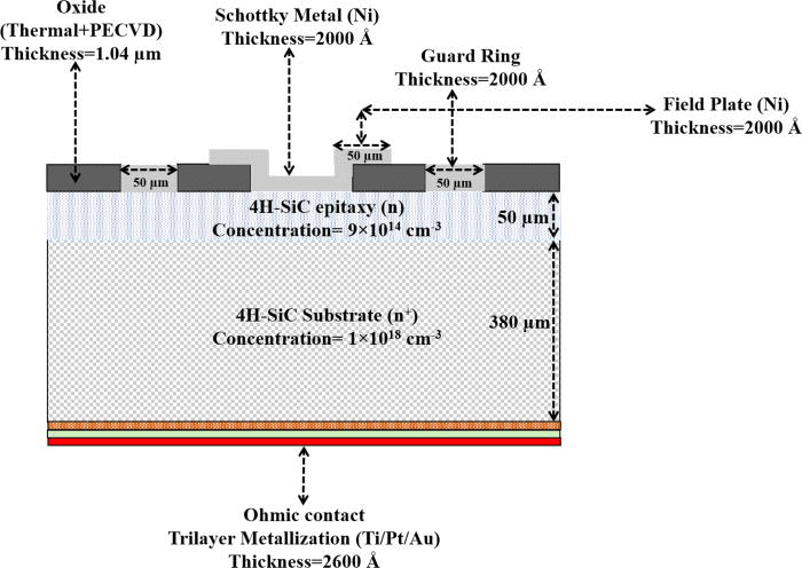
\includegraphics[width=0.7\textwidth]{figures/schottky_fabricacion.png}
\end{figure}
    
\end{frame}


\begin{frame}{Curva característica del diodo Schottky}

Cuando el diodo Schottky se polariza en directa, la corriente que fluye está dada por la ecuación:
%
\[ I_D = I_S (e^{\dfrac{V_A}{V_t}} - 1) \]

Donde $I_S$ es una constante que describe la corriente de fuga de reversa, y se denomina corriente de saturación del diodo.

\begin{figure}[H]
    \centering
    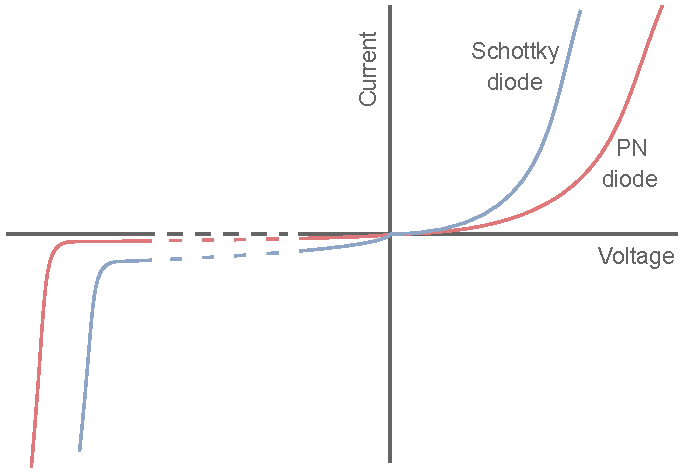
\includegraphics[width=0.5\textwidth]{figures/schottky_curva_transferencia.pdf}
\end{figure}

    
\end{frame}



\begin{frame}{Lecturas recomendadas}

\begin{itemize}
    \item Neudeck, G. (1993). El diodo PN de unión: Temas selectos de ingeniería (2da ed.).  Addison-Wesley Iberoamericana.
\end{itemize}

\end{frame}

\end{document}
